\chapter{Wstęp}

Świat jest odwzorowywany przez programy komputerowe za pomocą modeli.
Zawierają one uproszczoną reprezentację rzeczywistości, a logika programu
umożliwia wykonywanie obliczeń na podstawie modelu, jego modyfikację, lub
utrwalenie i udostępnienie do wglądu innym osobom.
Modele te mogą być prezentowane użytkownikowi na wiele sposobów. Jednym z nich
jest reprezentacja graficzna w~formie diagramu. Taka metoda reprezentacji
ozwala użytkownikowi na łatwiejsze zrozumienie modelu
oraz jego modyfikację, w porównaniu do~formatu tekstowego, ponieważ jest
wizualna i przestrzenna, a więc jest naturalniejszą formą dla mózgu człowieka.

Przykładem modeli z reprezentacją graficzną, które są zrozumiałe zarówno dla
człowieka, jak i maszyny, oraz
przydają się podczas wytwarzania oprogramowania, są modele korzystające
z~\gls{UML}~\cite{wikipedia-uml}. Przedstawiają
one strukturę klas w programie oraz zależności między klasami. Na ich podstawie
czytelnik może wysokopoziomowo zapoznać się~ze strukturą programu, a
odpowiednie narzędzia pozwolą wygenerować kod klas w danym języku
programowania, który może służyć jako początek do późniejszego rozwoju
aplikacji. Przykładowy model \gls{UML} został przedstawiony na
rysunku~\ref{rys:przykladowy-model-uml}.

\begin{figure}[!hb]
	\centering
	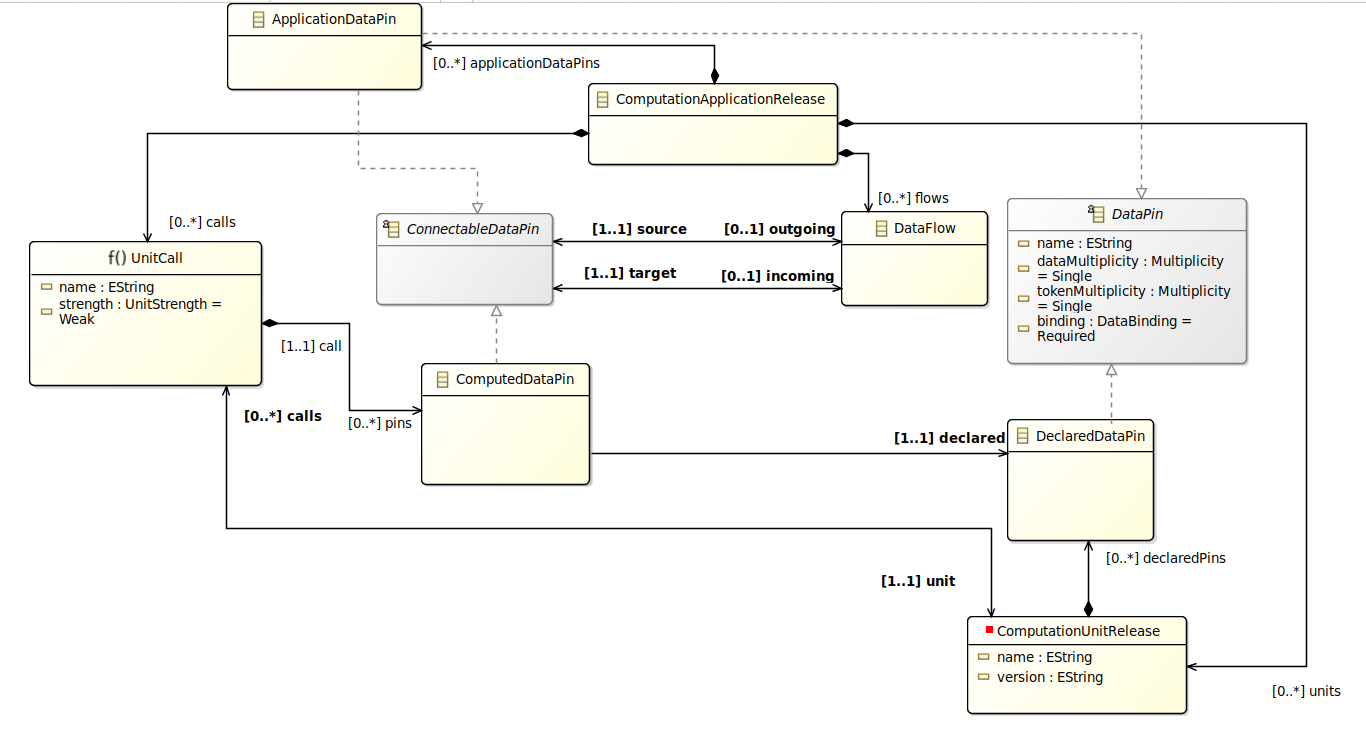
\includegraphics[width=0.95\linewidth]{./images/example-uml-model.png}
	\caption{Przykładowy model \gls{UML}.}\label{rys:przykladowy-model-uml}
\end{figure}

\gls{UML} jest przykładem uniwersalnego języka do opisu modeli klas programu.
Nie jest on~związany z żadną konkretną tematyką klas i pozwala na modelowanie
programów o~różnym zastosowaniu i przeznaczeniu. Istnieją także języki do opisu
modeli ściślej związanych z~konkretną dziedziną, czyli \gls{DSL}. Takie języki
są zazwyczaj mniejsze i mniej skomplikowane od języków uniwersalnych, a także
mają dokładniejszą semantykę (znaczenie elementów modelu). Potrafią więc one
odwzorować rzeczywistość w~sposób bardziej kompletny i zawrzeć więcej
szczegółów.

Strukturę samego modelu opisuje metamodel. Jest to model, który definiuje jakie
są~możliwe typy elementów modelu, jakie mają atrybuty, jak są połączone ze
sobą (składnia języka modelowania). Sam metamodel może być opisany na przykład
w języku UML\@ lub podobnym
bazowanym na nim, który będzie możliwiał wprowadzenie większej liczby
szczegółów. Taki metamodel często należy uzupełnić o zasady semantyczne ---
informacje o znaczeniu elementów, które nie mogą być zapisane w strukturze
metamodelu. Przykładową informacją semantyczną w modelu UML może być informacja
o krotności asocjacji.

\emph{BalticLSC} jest platformą do obliczeń rozproszonych wykonywaną z
inicjatywy
\emph{INTERREG Regionu Morza Bałtyckiego Unit Europejskiej}. Platforma ta
pozwala
wykonać obliczenia wykorzystując dostępne moduły obliczeniowe. Aplikacje
obliczeniowe definiowane są w postaci diagramów przedstawiających przepływ
danych między modułami obliczeniowymi. Przykład diagramu opisującego aplikację
obliczeniową został przedstawiony na
rysunku~\ref{rys:przykladowy-diagram-balticlsc}.  Model obliczeń opisany jest w
języku \gls{CAL}, który jest opisany za pomocą metamodelu~\cite{cal-metamodel}.

\begin{figure}[!hb]
	\centering

	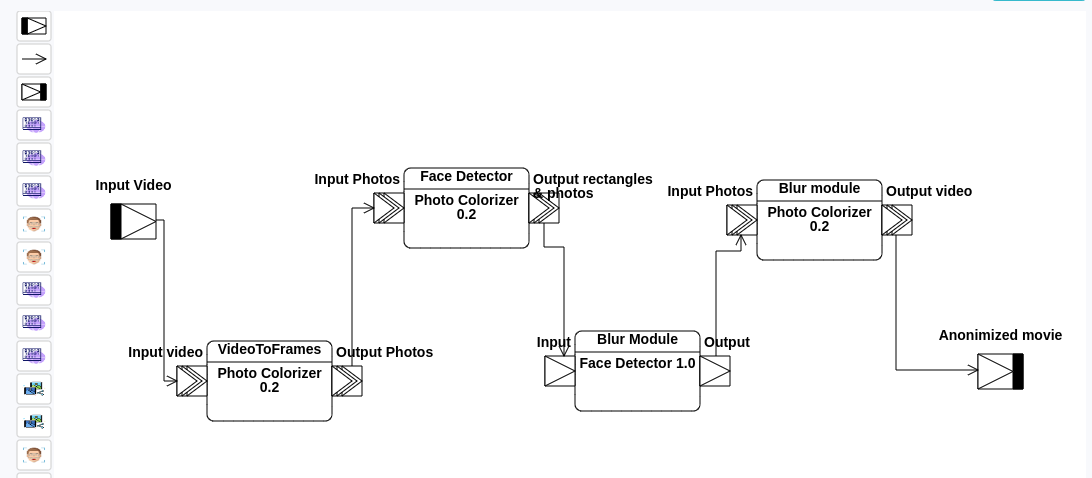
\includegraphics[width=0.95\linewidth]{./images/balticlsc-example-diagram.png}
	\caption{Przykładowy diagram przedstawiający aplikację obliczeniową w
		BalticLSC\@.}\label{rys:przykladowy-diagram-balticlsc}
\end{figure}

Istniejący edytor diagramów w BalticLSC dostępny jest jako część aplikacji
przeglądarkowej udostępnionej przez platformę. Do komunikacji z aplikacją
serwerową wykorzystuje inną reprezentację aplikacji obliczeniowej --- zapisuje
ją w postaci pudełek (prostokątów) oraz połączeń między nimi. Nie komunikuje
się on z aplikacją serwerową przesyłając informacje o strukturze modelu
zgodnej z metamodelem języka \gls{CAL}. Sprawia to, że po obu stronach (serwera
i aplikacji przeglądarkowej) potrzebne są dodatkowe transformacje
przetwarzające ogólny opis diagramu na model aplikacji obliczeniowej.

Sirius Web~\cite{sirius-web-github} jest narzędziem przygotowywanym przez firmę
Eclipse do tworzenia edytorów
diagramów działających w przeglądarce bazujących na metamodelach \gls{EMF}.
Technologia \gls{EMF} jest wykorzystywana od roku
2007~\cite{eclipse-sirius-wikipedia}, a metamodele
w~przeszłości mogły być tworzone używając oprogramowania Sirius
Desktop. Wykorzystując Sirius Web można w prosty sposób otrzymać aplikację
przeglądarkową umożliwiającą możliwości przeglądania i edycji modeli zbliżone
do tych,
które dotychczas oferowała jedynie aplikacja wymagająca instalacji na
komputerze użytkownika. Oprócz łatwiejszego dostępu do edytora diagramów dla
nowych użytkowników, wykorzystanie technologii przeglądarkowych do budowy
edytora diagramów pozwalają na dodanie mechanizmów kontroli dostępu do
wybranych modeli dla pewnych użytkowników, a także możliwości współpracy nad
modelem przez różne osoby w~czasie rzeczywistym.

W ustrukturyzowanym modelu zawierającym obiekty dziedzinowe w nietrudny sposób
można wyrazić reguły determinujące poprawność semantyczną modelu. Sirius
Desktop pozwala w tym zakresie na definiowanie semantycznych reguł
walidacyjnych, które są uruchamiane po każdej modyfikacji modelu i pokazują
błędnie umieszczone elementy. Odpowiednik tej funkcjonalności jest pożądany
także w edytorach diagramów opartych na Sirius Web.

W ramach tej pracy magisterskiej przygotowany został edytor diagramów dla
systemu BalticLSC korzystający z \emph{Sirius Web}. Edytor ten bazuje na
formalnym metamodelu \gls{EMF} opisującym język \gls{CAL} do
opisu aplikacji obliczeniowej. Ponadto, dostarczona została metoda sprawdzania
poprawności przygotowywanych przez użytkownika modeli na podstawie
zdefiniowanych reguł walidacji.

\section{Motywacja i cel pracy}

Jedną z alternatyw do wykorzystania Sirius Web do budowy edytora diagramów jest
wykorzystanie gotowych bibliotek JavaScript do wyświetlania i modyfikacji
diagramów (przykłady: \emph{react-diagrams}~\cite{react-diagrams-github},
\emph{Cytoscape.js}~\cite{cytoscape-js-homepage},
\emph{vis-network}~\cite{vis-network-github}). Są one ogólnymi narzędziami
pozwalającymi na zbudowanie własnego edytora diagramów. Dają sporą dowolność w
kwestii wyświetlania diagramu oraz
dostępnych funkcjonalności. Nie narzucają one
wykorzystania ustrukturyzowanych modeli poprzez wymaganie stworzenia
metamodelu. Z uwagi na swoją ogólność są trudniejsze do dostosowania do
własnych potrzeb, ponieważ funkcjonalności takie jak zapisywanie modeli w bazie
danych, współpraca w czasie rzeczywistym, walidacja modelu należy
zaimplementować samemu. Ponadto, modyfikacja takiego edytora diagramów wymaga
znajomości języka JavaScript.

Sirius Web dostarcza większość z tych
funkcjonalności wymagając jedynie wskazania metamodelu, który ma wykorzystywać.
Korzyści płynące z łatwego do przygotowania przeglądarkowego edytora diagramów
dla wybranych przez
nas modeli prezentują technologię Sirius Web jako interesującą i wartą użycia,
pomimo jej wczesnej fazy rozwoju i braku dokumentacji.

Celem tej pracy magisterskiej jest zbadanie możliwości udostępnianych przez
Sirius Web poprzez wykorzystanie go do przygotowania edytora
diagramów dla modeli języka CAL na platformie BalticLSC\@. Elementem edytora,
na który należy zwrócić szczególną uwagę, jest możliwosć walidacji modeli,
czyli weryfikacji ich~poprawności strukturalnej i semantycznej.

Ponadto, praca ta będzie jednym z pierwszych zastosowań Sirius Web wykonanych
przez osoby spoza zespołu budującego tą technologię, co może dostarczyć
dodatkowych informacji zwrotnych na temat prostoty jego wykorzystania, a także
napotkanych błędów i~niedociągnięć. Dla osób rozważających budowę edytora
modeli w oparciu o Sirius Web, praca ta będzie stanowiła źródło informacji o
wrażeniach z wykorzystania tej technologii, co pomoże podjąć bardziej świadomą
decyzję o używanych technologiach.
Z uwagi na brak dostępnej dokumentacji Sirius Web, praca ta może służyć również
jako przykład wykorzystania własnego metamodelu w tym edytorze diagramów.

Taki edytor diagramów bazujący na Sirius Web mógłby również zostać wykorzystany
w~aplikacji przeglądarkowej platformy BalticLSC\@. Jest on oparty o
ustrukturyzowany opis modelu, co pozwoliłoby na uproszczenie metody komunikacji
między serwerem aplikacyjnym a~aplikacją przeglądarkową, ponieważ nie byłyby
wymagane transformacje z aktualnego, ogólnego formatu danych do formatu
zgodnego z metamodelem.

\section{Zakres pracy}

W ramach pracy magisterskiej wykonano następujące czynności:

\begin{itemize}
	\item Stworzenie metamodelu języka \gls{CAL} w \gls{EMF}\@ z wykorzystaniem Sirius Desktop.
	\item Wykorzystanie tego metamodelu w Sirius Web. Zgłoszenie usterek autorom Sirius Web poprzez GitHub.
	\item Porównanie możliwości Sirius Web i Sirius Desktop. Zgłoszenie brakujących funkcjonalności autorom Sirius Web poprzez GitHub.
	\item Dodanie do metamodelu elementów usprawniających pracę z nim (automatyzacja niektórych czynności, dodanie ograniczeń utrudniających zrobienie błędu).
	\item Modyfikacja przeglądarkowego interfejsu użytkownika Sirius Web poprzez dodanie do niego przybornika z BalticLSC\@. Przybornik umożliwia w łatwy sposób dodanie nowych elementów do modelu.
	\item Dodanie mechanizmu walidacji semantycznej modelu sprawdzającego poprawność modelu z regułami zdefiniowanymi w języku Java.
	\item Stworzenie planu integracji rozwiązania z BalticLSC\@.
	\item Stworzenie przykładowej aplikacji przeglądarkowej zawierającej jedynie edytor diagramów z Sirius Web. Taki przykład pokazuje możliwość wykorzystania Sirius Web jako element innej aplikacji przeglądarkowej.
\end{itemize}

\vspace{1em}

\noindent Poza zakresem pracy pozostały następujące czynności:

\begin{itemize}
	\item Integracja stworzonego rozwiązania jako alternatywnego edytora diagramów dla systemu BalticLSC\@.
	\item Naprawa zgłoszonych usterek w Sirius Web.
\end{itemize}

\chapter{Tworzenie edytorów graficznych na bazie metamodeli}

\section{Metamodelowanie}

\section{Edytory graficzne na podstawie metamodeli}

\chapter{Metamodel dla języka CAL}

W tym rozdziale zostanie omówione przygotowane rozwiązanie.

\section{Język opisu obliczeń w BalticLSC}

\section{Stworzony metamodel EMF dla języka CAL}

Omówienie przygotowanego modelu. Zrzut ekranu przedstawiający model. Omówienie
elementów oraz jakie one mają przełożenie na wykonanie obliczeń przez
BalticLSC\@.

\subsection{Warunkowa zmiana stylu elementów}

Omówienie reguł warunkowej zmiany stylu elementów diagramu:

\begin{enumerate}
	\item \texttt{DataPin} zmieniają ikonę na podstawie swoich \textit{data
		      multiplicity} oraz \textit{token multiplicity}.
	\item \texttt{ComputedDataPin} zmieniają kolor na podstawie swojego
	      \textit{data binding}.
\end{enumerate}

\subsection{Narzędzia edytora diagramów}

Omówienie dodanych \textit{Tools} z Sirius:

\begin{itemize}
	\item usunięcie \texttt{UnitCall} lub \texttt{ApplicationDataPin} usuwa również powiązane \texttt{DataFlow}
	\item usunięcie \texttt{ComputedDataPin} z poziomu edytora diagramów nie jest możliwe
	\item ograniczenia na tworzenie \texttt{DataFlow} tak, aby były semantycznie poprawne
	\item automatyczne usuwanie i tworzenie \texttt{ComputedDataPin} po zmianie \texttt{ComputationUnitRelease} dla danego \texttt{UnitCall}
	\item okno dialogowe ułatwiające tworzenie \texttt{UnitCall} dla istniejącego \texttt{ComputationUnitRelease}
	\item \ldots
\end{itemize}

\subsection{Reguły walidacyjne powiązane z
	metamodelem}\label{sec:regulky-walidacyjne-metamodel}

Omówienie \textit{semantic validation rule} z pliku \texttt{*.odesign}, które
działają w Sirius Desktop.

\subsection{Testy metamodelu}

Omówienie dodanych testów jednostkowych modelu (głównie dotyczy automatycznego
zarządzania \texttt{ComputedDataPin} w zależnosci od
\texttt{ComputationUnitRelease} dla konkretnego \texttt{UnitCall}).

\chapter{Dostosowanie Sirius Web dla systemu BalticLSC}

\section{Użycie metamodelu języka CAL w Sirius Web}

Opis jak wykorzystać metamodel EMF w Sirius Web.

\begin{itemize}
	\item konfiguracja Maven
	\item odpowiednia modyfikacja klas Javy w Sirius Web
\end{itemize}

\noindent oraz jaki rezultat uzyskano.

\section{Integracja przybornika BalticLSC w Sirius Web}

Opis problemu dodawania nowych \texttt{UnitCall} do diagramu --- trzeba
zdefiniować \texttt{ComputationUnitRelease} w diagramie.

Rozwiązanie (zaczerpnięte z edytora diagramów BalticLSC) --- przybornik
(toolbox).

Opis jak to zrobiono, od strony backendu jak i frontendu. Omówienie trudności w
modyfikacji interfejsu użytkownika Sirius Web (trzeba było skopiować kod
źródłowy niektórych komponentów z biblioteki \textit{Sirius Components} do kodu
aplikacji Sirius Web, ponieważ komponenty te nie umożliwiały modyfikacji
interfejsu i wstawiania do nich nowych elementów --- najlepiej dać zrzut ekranu
co można było łatwo zmienić, a co wymagało skopiowania kodu).

\section{Walidacja semantyczna modelu}

Informacja o informacjach diagnostycznych udostępnianych domyślnie przez Sirius
Web.

Brak uruchamiania reguł semantycznych zdefiniowanych w
metamodelu~\ref{sec:regulky-walidacyjne-metamodel}.

Opis dodanego rozwiązania (własne klasy Javowe które zwracają listę informacji
diagnostycznych, oraz strumieniowanie ich do przeglądarki wykorzystując
istniejące rozwiązanie do walidacji).

\section{Użycie edytora Sirius Web w BalticLSC}

Omówienie przygotowanego planu integracji.

\chapter{Ocena Sirius Web}

\section{Różnice między Sirius Web a Sirius Desktop}

Omówienie różnic oraz usterek zgłoszonych przeze mnie w repozytorium Sirius
Web.

\section{Użycie własnego metamodelu}

\section{Dodawanie funkcjonalności do edytora}

\chapter{Informacje techniczne}

\section{Wykorzystane biblioteki}

Tabela z wykorzystywanymi bibliotekami i ich licencjami.

\section{Projekt systemu}

Diagram z backendami oraz frontendami BalticLSC, a także bazą danych
PostgreSQL\@.

\section{Projekt modułów}

Informacje o modułach backendu (projekty Javy w Sirius Web).

\section{Instrukcja wdrożenia}

\subsection{Wymagania}

Docker, lub Java 11, Maven, PostgreSQL

\subsection{Instrukcja instalacji}

Opis: albo Docker, albo instalacja manualna (potwórzenie instrukcji z
\texttt{README.md}).

\subsection{Instrukcja uruchomienia}

Opis: albo Docker, albo manualnie uruchomienie serwera

\section{Instrukcja użycia}

Jak użyć aplikacji do stworzenia prostego modelu

Powinno także zawierać informacje o logowaniu się do BalticLSC\@.

\section{Instrukcja utrzymania}

\subsection{Kopia zapasowa bazy danych}

Jak stworzyć kopię bazy w PostgreSQL\@?

\subsection{Aktualizowanie wersji Sirius Web}

Opis metody aplikowania najnowszych zmian z repozytorium Sirius Web
(generowanie \texttt{git patch} i aplikowanie ich).

\section{Zabezpieczenia}

Brak zabezpieczeń.

\section{Testy akceptacyjne rozwiązania}

Opis kilku testów, które użytkownik może chcieć wykonać aby sprawdzić, czy
rozwiązanie działa poprawnie.

\subsection{Wynik testów akceptacyjnych}

Czy się udały?

\chapter{Podsumowanie}

\section{Wyniki pracy}

Co zostało osiągnięte? Czy cel został zdobyty?

\section{Wnioski}

Sirius Web jest w fazie rozwoju, ale można już go użyć. Brakuje dokumentacji,
więc wymagany jest \textit{reverse engineering}, czytanie kodu źródłowego,
metoda prób i błędów, debuggowanie aplikacji, zgłaszanie usterek lub zadawanie
pytań w repozytorium projektu.

Występują różnice między Sirius Web a Sirius Desktop.

\section{Możliwości na rozwój}

Wymienić co można zrobić dalej:

\begin{itemize}
	\item integracja z BalticLSC
	\item dodanie większej liczby reguł walidacji semantycznej
\end{itemize}

\section{Sekcje, o których pomyślałem, ale pomijam}\label{sec:pominiete-sekcje}

W tej sekcji wymienię sekcje, o których pomyślałem, że mogą się znaleźć w pracy
magisterskiej. Ostatecznie chciabym je pominąć ze względu na charakter pracy
--- praca jest badawcza, a nie polegała na wytworzeniu nowego oprogramowania.
Pominięte sekcje to:

\begin{enumerate}
	\item wykorzystana metoda wytwarzania oprogramowania
	\item FURPS (wymagania funkcjonalne i niefunkcjonalne)
\end{enumerate}

Ta sekcja (\ref{sec:pominiete-sekcje}) zostanie usunięta z pracy magisterskiej
i służy tylko ułatwieniu komunikacji z promotorem w sprawie ustalenia nagłówków
sekcji pracy magisterskiej.
